\section{Problem Statement}
%We define the problem of path planning as follows: Given a start point and an end point, find the ``best'' path between them, where the definition of ``best'' depends on a set of preferences. Traditionally, the selected path will depend on two things: the location of obstacles and the length of the path, i.e. the planned paths are generally the shortest path to the goal that avoids collisions with any other objects. Finding such a path is generally easy. However, beyond avoiding collisions and getting to the destination efficiently, there are a number of other factors that can factor into which path is considered ``best.'' 

Non-lethal path planning involves finding the path from a start to a goal while minimizing the total cost from the costmap and the accumulated totals of the path constant. The duality of maximizing the one quantity while minimizing the other results in a continuum of different paths that could be considered optimal depending on the weighting of the two sides. 

%\begin{figure}
%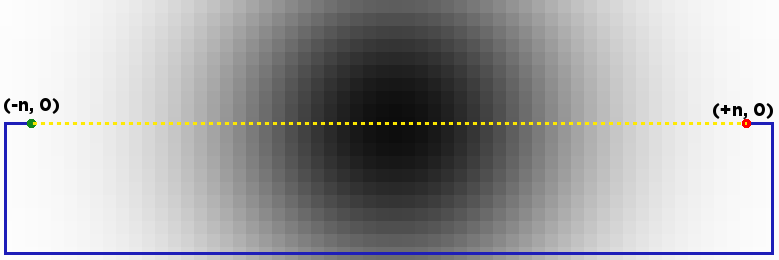
\includegraphics[width=\columnwidth]{graphix/TwoPaths.png}
%\caption{Two Simple Paths - The dotted yellow path is the shortest possible path. The solid blue path is the path with the lowest possible cost (within the bounds of the costmap). The tint of each cell is proportional to its cost. The green and red dots indicate the start and goal points respectively. }
%\label{fig:twopaths}
%\end{figure}

%The prioritization is separated into two different subsystems. First, there is the costmap where the value of the cells is stored. If only the

%If we prioritize the shortest possible path (as most planners do), we end up with the straight path seen in Figure \ref{fig:twopaths}, which does not make any attempt to avoid the obstacle. (Note that there are no lethal obstacles shown in the figure.) However, the lowest cost regions are along the border of the costmap, so if lowest cost becomes the priority, a longer more round-about path will be taken. 

\begin{figure}
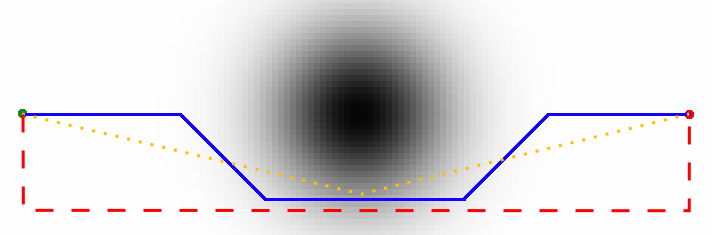
\includegraphics[width=\columnwidth]{graphix/connectedness.png}
\caption{Three Paths with Difference Cell Connectivity - The most general case (shown as a dotted yellow line) allows the robot to move at arbitrary angles in the grid. A more restricted case (shown as a solid blue line) allows for travel parallel with the grid and on the diagonals. The simplest case (shown with a dashed red line) allows for paths only parallel to the grid's axes. }
\label{fig:connectedness}
\end{figure}

One major factor that shapes the paths is the connectivity of the cells in the costmap, as seen in Figure \ref{fig:connectedness}. In the most general case, the paths can be at any angle, which can result in the shortest paths but takes longer to calculate. It's easier to calculate the optimum path if you only consider the cell's immediate neighbors. Moving to any of the cell's eight neighbors (the Moore neighborhood) allows for horizontal, vertical and diagonal moves. Moving to one of the cell's four immediate neighbors (the von Neumann neighborhood) results in only horizontal and vertical movement. Since the first two options would require scaling each cell's costs to be proportional to the distance traveled in the cell, and to make the math more tractable for this initial analysis, we are limiting ourselves to only consider paths in the 4-connected graph. 

A formal statement of the problem includes the following elements. First, we define a grid of discretized cells lying in a two dimensional plane, denoted by $x$ and $y$. Each cell has a non-negative cost, denoted by $f(x,y)$, where all cells with $f(x,y)\ge L$ are considered to be lethal, and the rest are non-lethal or free. Thus, we are trying to find the following:
\begin{equation}
   \displaystyle
 \min_{\forall \mathrm{path} p} C(p) = \min_{\forall \mathrm{path} p} \sum\limits_{(x,y) \in p}^{} \Big[ f(x,y) + P \Big] 
 \end{equation}
where $C(p)$ represents the combination of the path length and summation of $f(x,y)$, and $P$ is the path constant. This ensures that we are minimizing both the costmap cost plus the constant value for each cell entered.

For purposes of this paper, let us further refine the problem to reduce the number of cases we must consider. First, let us consider paths that go from $(-n, 0)$ to $(n, 0)$. This means that the costmap will be aligned to the primary direction of travel (i.e. the shortest path passes through $2n$ cells. If they were unaligned, the paths would be substantially different in shape, and would require analysis beyond the scope of this paper. 

We further assume that there are no lethal cells in our costmap, since path planning algorithms already do a fine job of avoiding lethal obstacles. Ergo, for now, we can presume that any non-lethal plan is a repeated application of planning with only non-lethal obstacles. 


